\documentclass[10pt, xcolors={RGB}, hyperref={pdfpagelabels=false,
        colorlinks=true,
        linkcolor=black,
        urlcolor=black,
        citecolor=black,
        filecolor=black,
        menucolor=black,
        pdftex=true,
        bookmarks=true,
        bookmarksopen=true,
        hyperfootnotes=true}]{beamer}
\pdfpageattr{/Group << /S /Transparency /I true /CS /DeviceRGB>>}
\usepackage[T1]{fontenc}
\usepackage[utf8]{inputenc}
\usepackage{graphicx}
\usepackage{tabularx}
\usepackage{multirow}

\usepackage{pifont}
\usepackage{multicol}

\usepackage{setspace}
\renewcommand{\baselinestretch}{1.25}

\usepackage{helvet}
\renewcommand{\familydefault}{\sfdefault}

\definecolor{dodgerblue}{RGB}{30,144,255}
\definecolor{springgreen3}{RGB}{0,139,69}
\definecolor{springgreen2}{RGB}{0,205,102}
\definecolor{firebrick2}{RGB}{238,44,44}
\definecolor{maroon2}{RGB}{238,48,167}
\definecolor{goldenrod2}{RGB}{238,180,34}
\definecolor{deepskyblue}{RGB}{0,191,255}

\newif\ifblacked\blackedfalse
\ifblacked
    \hypersetup{%
        linkcolor=black,
        urlcolor=black,
        citecolor=black,
        filecolor=black,
        menucolor=black}
    \renewcommand{\thefootnote}{\textcolor{black}{\arabic{footnote}}}
\else
    \hypersetup{%
        linkcolor=dodgerblue,
        urlcolor=firebrick2,
        citecolor=springgreen3,
        filecolor=goldenrod2,
        menucolor=dodgerblue,
        bookmarksopen=true}
    \renewcommand{\thefootnote}{\textcolor{maroon2}{\arabic{footnote}}}
\fi

\usetheme{CambridgeUS}
\useoutertheme{infolines}
\useinnertheme{rectangles}
\setbeamercolor{frametitle}{fg=white, bg=springgreen3!90!black!60!white}
\setbeamercolor{title}{fg=white, bg=springgreen3!50!white}
\setbeamercolor{palette primary}{fg=springgreen3!40!black, bg=springgreen3!50!white}
\setbeamercolor{palette secondary}{fg=springgreen3!30!black, bg=springgreen3!70!white}
\setbeamercolor{palette tertiary}{fg=springgreen3!20!black, bg=springgreen3!90!white}
\setbeamercolor{structure}{fg=springgreen3!70!white}
\setbeamercolor{background canvas}{bg=white}
\setbeamercolor{normal text}{fg=black}
\setbeamercolor{block title}{bg=dodgerblue, fg=white!75!dodgerblue}
\setbeamercolor{example text}{fg=springgreen3}
\setbeamercolor{block title example}{bg=springgreen3, fg=white!75!springgreen3}
\setbeamercolor{alerted text}{fg=firebrick2}
\setbeamercolor{block title alerted}{bg=firebrick2, fg=white!75!firebrick2}

\usepackage{textcomp}
\usepackage{listings}
\usepackage{courier}
\lstset{ %
    backgroundcolor=\color{dodgerblue!2.5!white},       % choose the background color; you must add \usepackage{color} or \usepackage{xcolor}
    basicstyle={\tiny\ttfamily\mdseries},               % the size of the fonts that are used for the code
    breakatwhitespace=true,                             % sets if automatic breaks should only happen at whitespace
    breaklines=true,                                    % sets automatic line breaking
    captionpos=none,                                       % sets the caption-position to bottom
    commentstyle=\color{springgreen3},                  % comment style
    deletekeywords={...},                               % if you want to delete keywords from the given language
    escapeinside={!*}{*!},                              % if you want to add LaTeX within your code
    extendedchars=true,                                 % lets you use non-ASCII characters; for 8-bits encodings only, does not work with UTF-8
    frame=single,                                       % adds a frame around the code
    keepspaces=true,                                    % keeps spaces in text, useful for keeping indentation of code (possibly needs columns=flexible)
    keywordstyle={\color{dodgerblue}\textbf},           % keyword style
    morekeywords={*,...},                               % if you want to add more keywords to the set
    numbers=none,                                       % where to put the line-numbers; possible values are (none, left, right)
    numbersep=10pt,                                     % how far the line-numbers are from the code
    numberstyle=\tiny\color{goldenrod2},                % the style that is used for the line-numbers
    rulecolor=\color{dodgerblue},                       % if not set, the frame-color may be changed on line-breaks within not-black text (e.g. comments (green here))
    showspaces=false,                                   % show spaces everywhere adding particular underscores; it overrides 'showstringspaces'
    showstringspaces=false,                             % underline spaces within strings only
    showtabs=false,                                     % show tabs within strings adding particular underscores
    stepnumber=1,                                       % the step between two line-numbers. If it's 1, each line will be numbered
    stringstyle=\color{maroon2},                        % string literal style
    tabsize=2,                                          % sets default tabsize to 2 spaces
    title=\lstname,                                     % show the filename of files included with \lstinputlisting; also try caption instead of title
    showlines=false,                                    % prints empty lines at the end of listings
    xleftmargin=9mm,                                    % The dimensions are used as extra margins on the left and right
    xrightmargin=9mm,
    upquote=true,
    lineskip=-0.05ex,                                   % Specifies additional space between lines in listings
    aboveskip=2ex,                                      % Define the space above and below displayed listings
    belowskip=4ex,                                      % Define the space above and below displayed listings
    literate=%
    {à}{{\`a}}1
    {è}{{\`e}}1
    {é}{{\'e}}1
    {ê}{{\^e}}1
}
\lstdefinelanguage{JuliaConsole}{
    morecomment=[l]{\#},
    backgroundcolor=\color{gray!2.5!white},             % choose the background color; you must add \usepackage{color} or \usepackage{xcolor}
    rulecolor=\color{gray!50!white},                    % if not set, the frame-color may be changed on line-breaks within not-black text (e.g. comments (green here))
    alsoletter={>},
    literate=%
    *{\$}{{{\color{black}\bfseries \$}}}1
    {julia>}{{{\color{black}\bfseries julia>}}}6
}
\lstdefinelanguage{Julia}{
    keywordsprefix=\@,
    morekeywords={
        exit, whos, edit, load, is, isa, isequal, typeof, tuple, ntuple, uid, hash, finalizer, convert, promote,
        subtype, typemin, typemax, realmin, realmax, sizeof, eps, promote_type, method_exists, applicable,
        invoke, dlopen, dlsym, system, error, throw, assert, new, Inf, Nan, pi, im, begin, while, for, in, return,
        break, continue, macro, quote, let, if, elseif, else, try, catch, end, bitstype, ccall, do, using, module,
        import, export, importall, baremodule, immutable, local, global, const, Bool, Int, Int8, Int16, Int32,
        Int64, Uint, Uint8, Uint16, Uint32, Uint64, Float32, Float64, Complex64, Complex128, Any, Nothing, None,
        function, type, typealias, abstract, include, require, names, info, warn
    },
    alsoletter={>},
    sensitive=true,
    morecomment=[l]{\#},
    morecomment=[s]{\#=}{=\#},
    morestring=[b]',
    morestring=[b]",
    literate=%
    *{0}{{{\color{goldenrod2}\textbf{0}}}}1
    {1}{{{\color{goldenrod2}\textbf{1}}}}1
    {2}{{{\color{goldenrod2}\textbf{2}}}}1
    {3}{{{\color{goldenrod2}\textbf{3}}}}1
    {4}{{{\color{goldenrod2}\textbf{4}}}}1
    {5}{{{\color{goldenrod2}\textbf{5}}}}1
    {6}{{{\color{goldenrod2}\textbf{6}}}}1
    {7}{{{\color{goldenrod2}\textbf{7}}}}1
    {8}{{{\color{goldenrod2}\textbf{8}}}}1
    {9}{{{\color{goldenrod2}\textbf{9}}}}1
    {0.0}{{{\color{goldenrod2}\textbf{0.0}}}}3
    {1.0}{{{\color{goldenrod2}\textbf{1.0}}}}3
    {2.0}{{{\color{goldenrod2}\textbf{2.0}}}}3
    {3.0}{{{\color{goldenrod2}\textbf{3.0}}}}3
    {4.0}{{{\color{goldenrod2}\textbf{4.0}}}}3
    {5.0}{{{\color{goldenrod2}\textbf{5.0}}}}3
    {6.0}{{{\color{goldenrod2}\textbf{6.0}}}}3
    {7.0}{{{\color{goldenrod2}\textbf{7.0}}}}3
    {8.0}{{{\color{goldenrod2}\textbf{8.0}}}}3
    {9.0}{{{\color{goldenrod2}\textbf{9.0}}}}3
    {0.1}{{{\color{goldenrod2}\textbf{0.1}}}}3
    {1.1}{{{\color{goldenrod2}\textbf{1.1}}}}3
    {2.1}{{{\color{goldenrod2}\textbf{2.1}}}}3
    {3.1}{{{\color{goldenrod2}\textbf{3.1}}}}3
    {4.1}{{{\color{goldenrod2}\textbf{4.1}}}}3
    {5.1}{{{\color{goldenrod2}\textbf{5.1}}}}3
    {6.1}{{{\color{goldenrod2}\textbf{6.1}}}}3
    {7.1}{{{\color{goldenrod2}\textbf{7.1}}}}3
    {8.1}{{{\color{goldenrod2}\textbf{8.1}}}}3
    {9.1}{{{\color{goldenrod2}\textbf{9.1}}}}3
    {0.2}{{{\color{goldenrod2}\textbf{0.2}}}}3
    {1.2}{{{\color{goldenrod2}\textbf{1.2}}}}3
    {2.2}{{{\color{goldenrod2}\textbf{2.2}}}}3
    {3.2}{{{\color{goldenrod2}\textbf{3.2}}}}3
    {4.2}{{{\color{goldenrod2}\textbf{4.2}}}}3
    {5.2}{{{\color{goldenrod2}\textbf{5.2}}}}3
    {6.2}{{{\color{goldenrod2}\textbf{6.2}}}}3
    {7.2}{{{\color{goldenrod2}\textbf{7.2}}}}3
    {8.2}{{{\color{goldenrod2}\textbf{8.2}}}}3
    {9.2}{{{\color{goldenrod2}\textbf{9.2}}}}3
    {0.3}{{{\color{goldenrod2}\textbf{0.3}}}}3
    {1.3}{{{\color{goldenrod2}\textbf{1.3}}}}3
    {2.3}{{{\color{goldenrod2}\textbf{2.3}}}}3
    {3.3}{{{\color{goldenrod2}\textbf{3.3}}}}3
    {4.3}{{{\color{goldenrod2}\textbf{4.3}}}}3
    {5.3}{{{\color{goldenrod2}\textbf{5.3}}}}3
    {6.3}{{{\color{goldenrod2}\textbf{6.3}}}}3
    {7.3}{{{\color{goldenrod2}\textbf{7.3}}}}3
    {8.3}{{{\color{goldenrod2}\textbf{8.3}}}}3
    {9.3}{{{\color{goldenrod2}\textbf{9.3}}}}3
    {0.4}{{{\color{goldenrod2}\textbf{0.4}}}}3
    {1.4}{{{\color{goldenrod2}\textbf{1.4}}}}3
    {2.4}{{{\color{goldenrod2}\textbf{2.4}}}}3
    {3.4}{{{\color{goldenrod2}\textbf{3.4}}}}3
    {4.4}{{{\color{goldenrod2}\textbf{4.4}}}}3
    {5.4}{{{\color{goldenrod2}\textbf{5.4}}}}3
    {6.4}{{{\color{goldenrod2}\textbf{6.4}}}}3
    {7.4}{{{\color{goldenrod2}\textbf{7.4}}}}3
    {8.4}{{{\color{goldenrod2}\textbf{8.4}}}}3
    {9.4}{{{\color{goldenrod2}\textbf{9.4}}}}3
    {0.5}{{{\color{goldenrod2}\textbf{0.5}}}}3
    {1.5}{{{\color{goldenrod2}\textbf{1.5}}}}3
    {2.5}{{{\color{goldenrod2}\textbf{2.5}}}}3
    {3.5}{{{\color{goldenrod2}\textbf{3.5}}}}3
    {4.5}{{{\color{goldenrod2}\textbf{4.5}}}}3
    {5.5}{{{\color{goldenrod2}\textbf{5.5}}}}3
    {6.5}{{{\color{goldenrod2}\textbf{6.5}}}}3
    {7.5}{{{\color{goldenrod2}\textbf{7.5}}}}3
    {8.5}{{{\color{goldenrod2}\textbf{8.5}}}}3
    {9.5}{{{\color{goldenrod2}\textbf{9.5}}}}3
    {0.6}{{{\color{goldenrod2}\textbf{0.6}}}}3
    {1.6}{{{\color{goldenrod2}\textbf{1.6}}}}3
    {2.6}{{{\color{goldenrod2}\textbf{2.6}}}}3
    {3.6}{{{\color{goldenrod2}\textbf{3.6}}}}3
    {4.6}{{{\color{goldenrod2}\textbf{4.6}}}}3
    {5.6}{{{\color{goldenrod2}\textbf{5.6}}}}3
    {6.6}{{{\color{goldenrod2}\textbf{6.6}}}}3
    {7.6}{{{\color{goldenrod2}\textbf{7.6}}}}3
    {8.6}{{{\color{goldenrod2}\textbf{8.6}}}}3
    {9.6}{{{\color{goldenrod2}\textbf{9.6}}}}3
    {0.7}{{{\color{goldenrod2}\textbf{0.7}}}}3
    {1.7}{{{\color{goldenrod2}\textbf{1.7}}}}3
    {2.7}{{{\color{goldenrod2}\textbf{2.7}}}}3
    {3.7}{{{\color{goldenrod2}\textbf{3.7}}}}3
    {4.7}{{{\color{goldenrod2}\textbf{4.7}}}}3
    {5.7}{{{\color{goldenrod2}\textbf{5.7}}}}3
    {6.7}{{{\color{goldenrod2}\textbf{6.7}}}}3
    {7.7}{{{\color{goldenrod2}\textbf{7.7}}}}3
    {8.7}{{{\color{goldenrod2}\textbf{8.7}}}}3
    {9.7}{{{\color{goldenrod2}\textbf{9.7}}}}3
    {0.8}{{{\color{goldenrod2}\textbf{0.8}}}}3
    {1.8}{{{\color{goldenrod2}\textbf{1.8}}}}3
    {2.8}{{{\color{goldenrod2}\textbf{2.8}}}}3
    {3.8}{{{\color{goldenrod2}\textbf{3.8}}}}3
    {4.8}{{{\color{goldenrod2}\textbf{4.8}}}}3
    {5.8}{{{\color{goldenrod2}\textbf{5.8}}}}3
    {6.8}{{{\color{goldenrod2}\textbf{6.8}}}}3
    {7.8}{{{\color{goldenrod2}\textbf{7.8}}}}3
    {8.8}{{{\color{goldenrod2}\textbf{8.8}}}}3
    {9.8}{{{\color{goldenrod2}\textbf{9.8}}}}3
    {0.9}{{{\color{goldenrod2}\textbf{0.9}}}}3
    {1.9}{{{\color{goldenrod2}\textbf{1.9}}}}3
    {2.9}{{{\color{goldenrod2}\textbf{2.9}}}}3
    {3.9}{{{\color{goldenrod2}\textbf{3.9}}}}3
    {4.9}{{{\color{goldenrod2}\textbf{4.9}}}}3
    {5.9}{{{\color{goldenrod2}\textbf{5.9}}}}3
    {6.9}{{{\color{goldenrod2}\textbf{6.9}}}}3
    {7.9}{{{\color{goldenrod2}\textbf{7.9}}}}3
    {8.9}{{{\color{goldenrod2}\textbf{8.9}}}}3
    {9.9}{{{\color{goldenrod2}\textbf{9.9}}}}3
    {Inf}{{{\color{goldenrod2}\textbf{Inf}}}}3
    {Int64}{{{\color{springgreen3}\textbf{Int64}}}}5
    {Float64}{{{\color{springgreen3}\textbf{Float64}}}}7
    {ASCIIString}{{{\color{springgreen3}\textbf{ASCIIString}}}}{11}
    {Char}{{{\color{springgreen3}\textbf{Char}}}}4
    {Bool}{{{\color{springgreen3}\textbf{Bool}}}}4
    {Any}{{{\color{springgreen3}\textbf{Any}}}}3
    {+}{{{\color{deepskyblue!85!black}\textbf{+}}}}1
    {-}{{{\color{deepskyblue!85!black}\textbf{-}}}}1
    {*}{{{\color{deepskyblue!85!black}\textbf{*}}}}1
    {/}{{{\color{deepskyblue!85!black}\textbf{/}}}}1
    {\%>\%}{{{\color{deepskyblue!85!black}\textbf{\%>\%}}}}3
    {R>}{{{\color{black}\bfseries R>}}}2
    {<-}{{{\color{black}\bfseries <-}}}2
    {(}{{{\color{deepskyblue!85!black}\textbf{(}}}}1
    {)}{{{\color{deepskyblue!85!black}\textbf{)}}}}1
    {[}{{{\color{deepskyblue!85!black}\textbf{[}}}}1
    {]}{{{\color{deepskyblue!85!black}\textbf{]}}}}1
    {\{}{{{\color{deepskyblue!85!black}\textbf{\{}}}}1
    {\}}{{{\color{deepskyblue!85!black}\textbf{\}}}}}1
    {julia>}{{{\color{black}\bfseries julia>}}}6
    {Pkg.status}{{{\color{dodgerblue}\textbf{Pkg.status}}}}{10}
    {Pkg.installed}{{{\color{dodgerblue}\textbf{Pkg.installed}}}}{13}
    {Pkg.update}{{{\color{dodgerblue}\textbf{Pkg.update}}}}{10}
    {Pkg.add}{{{\color{dodgerblue}\textbf{Pkg.add}}}}7
    {Pkg.clone}{{{\color{dodgerblue}\textbf{Pkg.clone}}}}9
    {Pkg.rm}{{{\color{dodgerblue}\textbf{Pkg.rm}}}}6
}
\lstdefinelanguage{Rconsole}{
    backgroundcolor=\color{gray!2.5!white},             % choose the background color; you must add \usepackage{color} or \usepackage{xcolor}
    rulecolor=\color{gray!50!white},                    % if not set, the frame-color may be changed on line-breaks within not-black text (e.g. comments (green here))
}
\lstdefinelanguage{R}{
    % backgroundcolor=\color{dodgerblue!2.5!white},       % choose the background color; you must add \usepackage{color} or \usepackage{xcolor}
    % rulecolor=\color{dodgerblue!50!white},              % if not set, the frame-color may be changed on line-breaks within not-black text (e.g. comments (green here))
    % commentstyle=\color{springgreen3},                  % comment style
    % keywordstyle={\color{dodgerblue}\textbf},           % keyword style
    % numberstyle=\scriptsize\color{goldenrod2},          % the style that is used for the line-numbers
    % stringstyle=\color{maroon2},                        % string literal style
    morekeywords={
        if, else, repeat, while, function, for, in, next, break, TRUE, FALSE, NULL, NA, NaN, abbreviate, abline, abs, acf, acos, acosh, addmargins, aggregate, agrep,
        alarm, alias, alist, all, anova, any, aov, aperm, append, apply, approx, approxfun, apropos, ar, args, arima, array, arrows, asin, asinh, assign, assocplot, atan,
        atanh, attach, attr, attributes, autoload, autoloader, ave, axis, backsolve, barplot, basename, beta, bindtextdomain, binomial, biplot, bitmap, bmp, body, box,
        boxplot, bquote, break, browser, builtins, bxp, by, bzfile, c call, cancor, capabilities, casefold, cat, category, cbind, ccf, ceiling, character, charmatch,
        chartr, chol, choose, chull, citation, class, close, cm, cmdscale, codes, coef, coefficients, col, colnames, colors, colorspaces, colours, comment, complex,
        confint, conflicts, contour, contrasts, contributors, convolve, cophenetic, coplot, cor, cos, cosh, cov, covratio, cpgram, crossprod, cummax, cummin, cumprod,
        cumsum, curve, cut, cutree, cycle, data, dataentry, date, dbeta, dbinom, dcauchy, dchisq, de, debug, debugger, decompose, delay, deltat, demo, dendrapply,
        density, deparse, deriv, det, detach, determinant, deviance, dexp, df, dfbeta, dfbetas, dffits, dgamma, dgeom, dget, dhyper, diag, diff, diffinv, difftime,
        digamma, dim, dimnames, dir, dirname, dist, dlnorm, dlogis, dmultinom, dnbinom, dnorm, dotchart, double, dpois, dput, drop, dsignrank, dt, dump, dunif, duplicated,
        dweibull, dwilcox, eapply, ecdf, edit, effects, eigen, emacs, embed, end, environment, eval, evalq, example, exists, exp, expression, factanal, factor, factorial,
        family, fft, fifo, file, filter, find, fitted, fivenum, fix, floor, flush, for, force, formals, format, formula, forwardsolve, fourfoldplot, frame, frequency,
        ftable, function, gamma, gaussian, gc, gcinfo, gctorture, get, getenv, geterrmessage, gettext, gettextf, getwd, gl, glm, globalenv, gray, grep, grey, grid, gsub,
        gzcon, gzfile, hat, hatvalues, hcl, hclust, head, heatmap, help, hist, history, hsv, httpclient, iconv, iconvlist, identical, identify, if, ifelse, image,
        influence, inherits, integer, integrate, interaction, interactive, intersect, invisible, isoreg, jitter, jpeg, julian, kappa, kernapply, kernel, kmeans, knots,
        kronecker, ksmooth, labels, lag, lapply, layout, lbeta, lchoose, lcm, legend, length, letters, levels, lfactorial, lgamma, library, licence, license, line, lines,
        list, lm, load, loadhistory, loadings, local, locator, loess, log, logb, logical, loglin, lowess, ls, lsfit, machine, mad, mahalanobis, makepredictcall, manova,
        mapply, match, matlines, matplot, matpoints, matrix, max, mean, median, medpolish, menu, merge, message, methods, mget, min, missing, mode, monthplot, months,
        mosaicplot, mtext, mvfft, names, napredict, naprint, naresid, nargs, nchar, ncol, next, nextn, ngettext, nlevels, nlm, nls, noquote, nrow, numeric, objects, offset,
        open, optim, optimise, optimize, options, order, ordered, outer, pacf, page, pairlist, pairs, palette, par, parse, paste, pbeta, pbinom, pbirthday, pcauchy, pchisq,
        pdf, pentagamma, person, persp, pexp, pf, pgamma, pgeom, phyper, pi, pico, pictex, pie, piechart, pipe, plclust, plnorm, plogis, plot, pmatch, pmax, pmin, pnbinom,
        png, pnorm, points, poisson, poly, polygon, polym, polyroot, postscript, power, ppoints, ppois, ppr, prcomp, predict, preplot, pretty, princomp, print, prmatrix,
        prod, profile, profiler, proj, promax, prompt, provide, psigamma, psignrank, pt, ptukey, punif, pweibull, pwilcox, q qbeta, qbinom, qbirthday, qcauchy, qchisq, qexp,
        qf, qgamma, qgeom, qhyper, qlnorm, qlogis, qnbinom, qnorm, qpois, qqline, qqnorm, qqplot, qr, qsignrank, qt, qtukey, quantile, quarters, quasi, quasibinomial,
        quasipoisson, quit, qunif, quote, qweibull, qwilcox, rainbow, range, rank, raw, rbeta, rbind, rbinom, rcauchy, rchisq, readline, real, recover, rect, reformulate,
        regexpr, relevel, remove, reorder, rep, repeat, replace, replicate, replications, require, reshape, resid, residuals, restart, return, rev, rexp, rf, rgamma, rgb,
        rgeom, rhyper, rle, rlnorm, rlogis, rm, rmultinom, rnbinom, rnorm, round, row, rownames, rowsum, rpois, rsignrank, rstandard, rstudent, rt, rug, runif, runmed,
        rweibull, rwilcox, sample, sapply, save, savehistory, scale, scan, screen, screeplot, sd, search, searchpaths, seek, segments, seq, sequence, serialize, setdiff,
        setequal, setwd, shell, sign, signif, sin, single, sinh, sink, smooth, solve, sort, source, spectrum, spline, splinefun, split, sprintf, sqrt, stack, stars, start,
        stderr, stdin, stdout, stem, step, stepfun, stl, stop, stopifnot, str, strftime, strheight, stripchart, strptime, strsplit, strtrim, structure, strwidth, strwrap,
        sub, subset, substitute, substr, substring, sum, summary, sunflowerplot, supsmu, svd, sweep, switch, symbols, symnum, system, t table, tabulate, tail, tan, tanh,
        tapply, tempdir, tempfile, termplot, terms, tetragamma, text, time, title, toeplitz, tolower, topenv, toupper, trace, traceback, transform, trigamma, trunc,
        truncate, try, ts, tsdiag, tsp, typeof, unclass, undebug, union, unique, uniroot, unix, unlink, unlist, unname, unserialize, unsplit, unstack, untrace, unz,
        update, upgrade, url, var, varimax, vcov, vector, version, vi, vignette, warning, warnings, weekdays, weights, which, while, window, windows, with, write,
        wsbrowser, xedit, xemacs, xfig, xinch, xor, xtabs, xyinch, yinch, zapsmall,
        ggplot, ggvis
    },
    sensitive=true,
    morecomment=[l]{\#},
    morestring=[b]',
    morestring=[b]",
    literate=%
    *{0}{{{\color{goldenrod2}\textbf{0}}}}1
    {1}{{{\color{goldenrod2}\textbf{1}}}}1
    {2}{{{\color{goldenrod2}\textbf{2}}}}1
    {3}{{{\color{goldenrod2}\textbf{3}}}}1
    {4}{{{\color{goldenrod2}\textbf{4}}}}1
    {5}{{{\color{goldenrod2}\textbf{5}}}}1
    {6}{{{\color{goldenrod2}\textbf{6}}}}1
    {7}{{{\color{goldenrod2}\textbf{7}}}}1
    {8}{{{\color{goldenrod2}\textbf{8}}}}1
    {9}{{{\color{goldenrod2}\textbf{9}}}}1
    {0.0}{{{\color{goldenrod2}\textbf{0.0}}}}3
    {1.0}{{{\color{goldenrod2}\textbf{1.0}}}}3
    {2.0}{{{\color{goldenrod2}\textbf{2.0}}}}3
    {3.0}{{{\color{goldenrod2}\textbf{3.0}}}}3
    {4.0}{{{\color{goldenrod2}\textbf{4.0}}}}3
    {5.0}{{{\color{goldenrod2}\textbf{5.0}}}}3
    {6.0}{{{\color{goldenrod2}\textbf{6.0}}}}3
    {7.0}{{{\color{goldenrod2}\textbf{7.0}}}}3
    {8.0}{{{\color{goldenrod2}\textbf{8.0}}}}3
    {9.0}{{{\color{goldenrod2}\textbf{9.0}}}}3
    {0.1}{{{\color{goldenrod2}\textbf{0.1}}}}3
    {1.1}{{{\color{goldenrod2}\textbf{1.1}}}}3
    {2.1}{{{\color{goldenrod2}\textbf{2.1}}}}3
    {3.1}{{{\color{goldenrod2}\textbf{3.1}}}}3
    {4.1}{{{\color{goldenrod2}\textbf{4.1}}}}3
    {5.1}{{{\color{goldenrod2}\textbf{5.1}}}}3
    {6.1}{{{\color{goldenrod2}\textbf{6.1}}}}3
    {7.1}{{{\color{goldenrod2}\textbf{7.1}}}}3
    {8.1}{{{\color{goldenrod2}\textbf{8.1}}}}3
    {9.1}{{{\color{goldenrod2}\textbf{9.1}}}}3
    {0.2}{{{\color{goldenrod2}\textbf{0.2}}}}3
    {1.2}{{{\color{goldenrod2}\textbf{1.2}}}}3
    {2.2}{{{\color{goldenrod2}\textbf{2.2}}}}3
    {3.2}{{{\color{goldenrod2}\textbf{3.2}}}}3
    {4.2}{{{\color{goldenrod2}\textbf{4.2}}}}3
    {5.2}{{{\color{goldenrod2}\textbf{5.2}}}}3
    {6.2}{{{\color{goldenrod2}\textbf{6.2}}}}3
    {7.2}{{{\color{goldenrod2}\textbf{7.2}}}}3
    {8.2}{{{\color{goldenrod2}\textbf{8.2}}}}3
    {9.2}{{{\color{goldenrod2}\textbf{9.2}}}}3
    {0.3}{{{\color{goldenrod2}\textbf{0.3}}}}3
    {1.3}{{{\color{goldenrod2}\textbf{1.3}}}}3
    {2.3}{{{\color{goldenrod2}\textbf{2.3}}}}3
    {3.3}{{{\color{goldenrod2}\textbf{3.3}}}}3
    {4.3}{{{\color{goldenrod2}\textbf{4.3}}}}3
    {5.3}{{{\color{goldenrod2}\textbf{5.3}}}}3
    {6.3}{{{\color{goldenrod2}\textbf{6.3}}}}3
    {7.3}{{{\color{goldenrod2}\textbf{7.3}}}}3
    {8.3}{{{\color{goldenrod2}\textbf{8.3}}}}3
    {9.3}{{{\color{goldenrod2}\textbf{9.3}}}}3
    {0.4}{{{\color{goldenrod2}\textbf{0.4}}}}3
    {1.4}{{{\color{goldenrod2}\textbf{1.4}}}}3
    {2.4}{{{\color{goldenrod2}\textbf{2.4}}}}3
    {3.4}{{{\color{goldenrod2}\textbf{3.4}}}}3
    {4.4}{{{\color{goldenrod2}\textbf{4.4}}}}3
    {5.4}{{{\color{goldenrod2}\textbf{5.4}}}}3
    {6.4}{{{\color{goldenrod2}\textbf{6.4}}}}3
    {7.4}{{{\color{goldenrod2}\textbf{7.4}}}}3
    {8.4}{{{\color{goldenrod2}\textbf{8.4}}}}3
    {9.4}{{{\color{goldenrod2}\textbf{9.4}}}}3
    {0.5}{{{\color{goldenrod2}\textbf{0.5}}}}3
    {1.5}{{{\color{goldenrod2}\textbf{1.5}}}}3
    {2.5}{{{\color{goldenrod2}\textbf{2.5}}}}3
    {3.5}{{{\color{goldenrod2}\textbf{3.5}}}}3
    {4.5}{{{\color{goldenrod2}\textbf{4.5}}}}3
    {5.5}{{{\color{goldenrod2}\textbf{5.5}}}}3
    {6.5}{{{\color{goldenrod2}\textbf{6.5}}}}3
    {7.5}{{{\color{goldenrod2}\textbf{7.5}}}}3
    {8.5}{{{\color{goldenrod2}\textbf{8.5}}}}3
    {9.5}{{{\color{goldenrod2}\textbf{9.5}}}}3
    {0.6}{{{\color{goldenrod2}\textbf{0.6}}}}3
    {1.6}{{{\color{goldenrod2}\textbf{1.6}}}}3
    {2.6}{{{\color{goldenrod2}\textbf{2.6}}}}3
    {3.6}{{{\color{goldenrod2}\textbf{3.6}}}}3
    {4.6}{{{\color{goldenrod2}\textbf{4.6}}}}3
    {5.6}{{{\color{goldenrod2}\textbf{5.6}}}}3
    {6.6}{{{\color{goldenrod2}\textbf{6.6}}}}3
    {7.6}{{{\color{goldenrod2}\textbf{7.6}}}}3
    {8.6}{{{\color{goldenrod2}\textbf{8.6}}}}3
    {9.6}{{{\color{goldenrod2}\textbf{9.6}}}}3
    {0.7}{{{\color{goldenrod2}\textbf{0.7}}}}3
    {1.7}{{{\color{goldenrod2}\textbf{1.7}}}}3
    {2.7}{{{\color{goldenrod2}\textbf{2.7}}}}3
    {3.7}{{{\color{goldenrod2}\textbf{3.7}}}}3
    {4.7}{{{\color{goldenrod2}\textbf{4.7}}}}3
    {5.7}{{{\color{goldenrod2}\textbf{5.7}}}}3
    {6.7}{{{\color{goldenrod2}\textbf{6.7}}}}3
    {7.7}{{{\color{goldenrod2}\textbf{7.7}}}}3
    {8.7}{{{\color{goldenrod2}\textbf{8.7}}}}3
    {9.7}{{{\color{goldenrod2}\textbf{9.7}}}}3
    {0.8}{{{\color{goldenrod2}\textbf{0.8}}}}3
    {1.8}{{{\color{goldenrod2}\textbf{1.8}}}}3
    {2.8}{{{\color{goldenrod2}\textbf{2.8}}}}3
    {3.8}{{{\color{goldenrod2}\textbf{3.8}}}}3
    {4.8}{{{\color{goldenrod2}\textbf{4.8}}}}3
    {5.8}{{{\color{goldenrod2}\textbf{5.8}}}}3
    {6.8}{{{\color{goldenrod2}\textbf{6.8}}}}3
    {7.8}{{{\color{goldenrod2}\textbf{7.8}}}}3
    {8.8}{{{\color{goldenrod2}\textbf{8.8}}}}3
    {9.8}{{{\color{goldenrod2}\textbf{9.8}}}}3
    {0.9}{{{\color{goldenrod2}\textbf{0.9}}}}3
    {1.9}{{{\color{goldenrod2}\textbf{1.9}}}}3
    {2.9}{{{\color{goldenrod2}\textbf{2.9}}}}3
    {3.9}{{{\color{goldenrod2}\textbf{3.9}}}}3
    {4.9}{{{\color{goldenrod2}\textbf{4.9}}}}3
    {5.9}{{{\color{goldenrod2}\textbf{5.9}}}}3
    {6.9}{{{\color{goldenrod2}\textbf{6.9}}}}3
    {7.9}{{{\color{goldenrod2}\textbf{7.9}}}}3
    {8.9}{{{\color{goldenrod2}\textbf{8.9}}}}3
    {9.9}{{{\color{goldenrod2}\textbf{9.9}}}}3
    {Inf}{{{\color{goldenrod2}\textbf{Inf}}}}3
    {+}{{{\color{deepskyblue!85!black}\textbf{+}}}}1
    {-}{{{\color{deepskyblue!85!black}\textbf{-}}}}1
    {*}{{{\color{deepskyblue!85!black}\textbf{*}}}}1
    {/}{{{\color{deepskyblue!85!black}\textbf{/}}}}1
    {\%>\%}{{{\color{deepskyblue!85!black}\textbf{\%>\%}}}}3
    {R>}{{{\color{black}\bfseries R>}}}2
    {<-}{{{\color{black}\bfseries <-}}}2
    {(}{{{\color{deepskyblue!85!black}\textbf{(}}}}1
    {)}{{{\color{deepskyblue!85!black}\textbf{)}}}}1
    {[}{{{\color{deepskyblue!85!black}\textbf{[}}}}1
    {]}{{{\color{deepskyblue!85!black}\textbf{]}}}}1
    {\{}{{{\color{deepskyblue!85!black}\textbf{\{}}}}1
    {\}}{{{\color{deepskyblue!85!black}\textbf{\}}}}}1
}
\lstdefinelanguage{md}{
    backgroundcolor=\color{dodgerblue!2.5!white},       % choose the background color; you must add \usepackage{color} or \usepackage{xcolor}
    rulecolor=\color{dodgerblue!50!white},              % if not set, the frame-color may be changed on line-breaks within not-black text (e.g. comments (green here))
    commentstyle=\color{springgreen3},                  % comment style
    keywordstyle={\color{dodgerblue}\textbf},           % keyword style
    numberstyle=\scriptsize\color{goldenrod2},          % the style that is used for the line-numbers
    stringstyle=\color{maroon2},                        % string literal style
    morecomment=[l][\color{dodgerblue}\textbf]{\#},
    sensitive=true,
    literate=%
    {à}{{\`a}}1
    {è}{{\`e}}1
    {é}{{\'e}}1
    {ê}{{\^e}}1
    {`}{{{\color{dodgerblue}\textbf{`}}}}1
    {*}{{{\color{dodgerblue}\textbf{*}}}}1
    {(}{{{\color{deepskyblue!85!black}\textbf{(}}}}1
    {)}{{{\color{deepskyblue!85!black}\textbf{)}}}}1
    {[}{{{\color{deepskyblue!85!black}\textbf{[}}}}1
    {]}{{{\color{deepskyblue!85!black}\textbf{]}}}}1
    {\{}{{{\color{deepskyblue!85!black}\textbf{\{}}}}1
    {\}}{{{\color{deepskyblue!85!black}\textbf{\}}}}}1
}
\lstdefinelanguage{yaml}{
    morecomment=[s]{<!--}{-->},
    morekeywords={
        output, word_document, html_document, pdf_document, beamer_presentation
    }
}
\usepackage{etoolbox}
\makeatletter
\patchcmd{\lsthk@SelectCharTable}{%
  \lst@ifbreaklines\lst@Def{`)}{\lst@breakProcessOther)}\fi
}{%
}{
}{
}
\makeatother

\setlength{\headheight}{15pt}
\setlength{\abovecaptionskip}{0pt}
\setlength{\tabcolsep}{10pt} % default

\newlength{\wideitemsep}
\setlength{\wideitemsep}{.5\itemsep}
\addtolength{\wideitemsep}{-7pt}
\let\olditem\item
\newcommand{\items}{\setlength{\itemsep}{\wideitemsep}\olditem}

\newcommand\bref[2]{\hyperref[#1]{#2~\ref*{#1}}}
\newcommand\cmd[1]{\texttt{\color{black}\textbf{#1}}}
\newcommand\cmdb[1]{\texttt{\color{dodgerblue}\textbf{#1}}}
\newcommand\cmdr[1]{\texttt{\color{firebrick2}\textbf{#1}}}
\newcommand\cmdg[1]{\texttt{\color{springgreen3}\textbf{#1}}}
\newcommand\cmdy[1]{\texttt{\color{goldenrod2}\textbf{#1}}}

\newenvironment{bquote}[1]
    {\begin{quotation}
    \vspace{10pt}
    \newcommand{\bqauthor}{\normalfont \begin{quote}\begin{flushright}--- #1\end{flushright}\end{quote}}
    \rmfamily \itshape {\huge\textbf{``}}
    }
    {{\huge\textbf{''}}
    \bqauthor
    \end{quotation}
    }

\usepackage[english, francais]{babel}
\selectlanguage{francais}

\AtBeginSection[]
{
  \begin{frame}
    \frametitle{Sommaire}
    \tableofcontents[sectionstyle=show/hide, subsectionstyle=show/hide/hide, subsubsectionstyle=hide/hide/hide]
  \end{frame}
}
% \AtBeginSubsection[]
% {
    % \begin{frame}
        % \frametitle{Sommaire}
        % \tableofcontents[sectionstyle=show/shaded, subsectionstyle=show/shaded/hide, subsubsectionstyle=show/shaded/hide]
    % \end{frame}
% }

\newcommand{\R}{\protect
\includegraphics[height=0.5cm, keepaspectratio]{./Logos/logo_R2.png}}
\newcommand{\Julia}{\protect{\raisebox{-0.5ex}{
\includegraphics[height=0.5cm, keepaspectratio]{./Logos/logo_julia.pdf}}}}
\newcommand{\Excel}{\protect{\raisebox{-0.5ex}{
\includegraphics[height=0.5cm, keepaspectratio]{./Logos/Logo_Microsoft_Excel_2013.png}}}}
\newcommand{\Word}{\protect{\raisebox{-0.5ex}{
\includegraphics[height=0.5cm, keepaspectratio]{./Logos/Logo_Microsoft_Word_2013.png}}}}
\newcommand{\Latex}{\protect{\raisebox{-0.8ex}{
\includegraphics[height=0.5cm, keepaspectratio]{./Logos/Logo_Latex.png}}}}

\date{\today}
\author[Mickaël Canouil]{\texorpdfstring{Mickaël Canouil\\ \vskip -0.25cm \href{mailto:mickael.canouil@cnrs.fr}{{\scriptsize mickael.canouil@cnrs.fr}}}{Mickaël Canouil}}
\institute[UMR 8199]{Génomique Intégrative et Modélisation des Maladies Métaboliques (CNRS UMR8199)\linebreak
            Institut de Biologie de Lille}
% \institute[UMR 8199]{Integrative Genomics and Modelization of Metabolic Diseases (CNRS UMR8199)\linebreak
            % Institut de Biologie de Lille}
\titlegraphic{
\includegraphics[height=1cm, keepaspectratio]{./Logos/logo_cnrs.pdf}\hspace{2cm}
\includegraphics[height=1cm, keepaspectratio]{./Logos/logo_egid.pdf}}


\title[\color{black}{Génération de documents avec }\protect{\raisebox{-0.25ex}{
\includegraphics[height=0.2cm, keepaspectratio]{./Logos/logo_R2.png}}}]{\texorpdfstring{Génération de documents avec {\R}}{Génération de documents avec R}}
\subtitle{xlsx, rmarkdown, knitr (et pandoc)}

% \graphicspath{{}}



\begin{document}
\maketitle

\begin{frame}
    \frametitle{Sommaire}
    \tableofcontents[sectionstyle=show/show, subsectionstyle=show/hide/hide, subsubsectionstyle=hide/hide/hide]
\end{frame}


\section{Générer un tableur Excel}
\subsection{Le package xlsx: un peu de lecture}
\begin{frame}[containsverbatim]{Le package xlsx: un peu de lecture (\cmdb{read.xlsx})}
\par{Le package xlsx propose une fonction de lecture fonctionnant sur le même principe que \cmdb{read.table}, avec un argument pour sélectionner la feuille Excel \Excel{}.}
\vspace{-2ex}
\begin{lstlisting}[language=R]
R> library(xlsx)
R> formalArgs(read.xlsx)
 [1] "file"          "sheetIndex"    "sheetName"     "rowIndex"
 [5] "startRow"      "endRow"        "colIndex"      "as.data.frame"
 [9] "header"        "colClasses"    "keepFormulas"  "encoding"
[13] "..."
\end{lstlisting}
\vspace{-2ex}
\begin{lstlisting}[language=R]
R> iris2 <- read.xlsx(file = "iris.xlsx", sheetIndex = 1, header = TRUE)
R> head(iris2)
  Sepal.Length Sepal.Width Petal.Length Petal.Width Species
1          5.1         3.5          1.4         0.2  setosa
2          4.9         3.0          1.4         0.2  setosa
3          4.7         3.2          1.3         0.2  setosa
4          4.6         3.1          1.5         0.2  setosa
5          5.0         3.6          1.4         0.2  setosa
6          5.4         3.9          1.7         0.4  setosa
\end{lstlisting}
\end{frame}


\subsection{Le package xlsx: un peu d'écriture}
\begin{frame}[containsverbatim]{Le package xlsx: un peu d'écriture (\cmdb{write.xlsx})}
\par{La fonction \cmdb{write.xlsx} s'utilise de la même façon que \cmdb{write.table}.}
\vspace{-2ex}
\begin{lstlisting}[language=R]
R> library(xlsx)
R> formalArgs(write.xlsx)
[1] "x"         "file"      "sheetName" "col.names" "row.names" "append"
[7] "showNA"
\end{lstlisting}
\vspace{-2ex}
\begin{lstlisting}[language=R]
R> write.xlsx(iris2, file = "iris.xlsx", row.names = FALSE)
\end{lstlisting}
\vspace{1ex}
\begin{center}
    \begin{figure}
        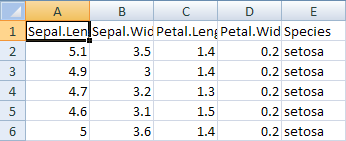
\includegraphics[height=1.7cm, keepaspectratio]{figures/iris_xlsx_1.png}
    \end{figure}
\end{center}
\end{frame}


\subsection{Le package xlsx: les accès}
\begin{frame}[containsverbatim]{Le package xlsx: les accès}
\begin{itemize}
\item \par{Créer ou charger un \cmdb{workbook} (Excel \Excel{} 2007):}
\vspace{-2ex}
\begin{lstlisting}[language=R]
R> wb <- createWorkbook(type = "xlsx")
R> wb <- loadWorkbook(file = "iris.xlsx")
\end{lstlisting}
\par{L'objet \cmdb{wb} est un objet S4 (champs accessibles avec \cmdb{@}) du package rjava.}
\vspace{4ex}
\item \par{Créer ou charger une feuille Excel \Excel{}:}
\vspace{-2ex}
\begin{lstlisting}[language=R]
R> sheet <- createSheet(wb, sheetName = "Sheet1")
R> sheet <- getSheets(wb)
\end{lstlisting}
\par{La fonction \cmdb{getSheets} renvoie un objet de type \cmdb{list}.
\\Chaque élément est une feuille Excel \Excel{}.}
\end{itemize}
\end{frame}


\subsection{Le package xlsx: la taille ça compte}
\begin{frame}[containsverbatim]{Le package xlsx: la taille ça compte}
\par{Redimensionner automatiquement les colonnes:}
\vspace{-2ex}
\begin{lstlisting}[language=R]
R> wb <- loadWorkbook(file = "iris.xlsx")
R> sheet <- getSheets(wb)[["Sheet1"]]
\end{lstlisting}
\vspace{-2ex}
\begin{lstlisting}[language=R]
R> autoSizeColumn(sheet, colIndex = seq(5)) # 5 colonnes dans les donnees iris
\end{lstlisting}
\vspace{2ex}
\par{Ne pas oublier de sauvegarder le \cmdb{workbook} avec \cmdb{saveWorkbook}.}
\vspace{-2ex}
\begin{lstlisting}[language=R]
R> saveWorkbook(wb, file = "iris.xlsx")
\end{lstlisting}
\vspace{1ex}
\begin{center}
    \begin{figure}
        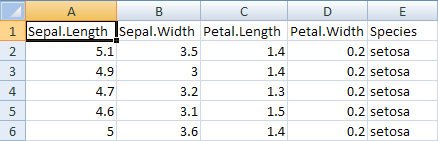
\includegraphics[height=1.7cm, keepaspectratio]{figures/iris_xlsx_2.png}
    \end{figure}
\end{center}
\end{frame}


\subsection{Le package xlsx: le style c'est important}
\begin{frame}[containsverbatim]{Le package xlsx: le style c'est important}
\par{Définition et application d'un style de cellule:}
\vspace{-2ex}
\begin{lstlisting}[language=R]
R> titleStyle <- CellStyle(wb,
       font = Font(wb, isBold = TRUE), # texte en gras
       alignment = Alignment(horizontal = "ALIGN_CENTER") # alignement horizontal du texte
   )
\end{lstlisting}
\vspace{-2ex}
\begin{lstlisting}[language=R]
R> rows  <- getRows(sheet, rowIndex = 1) # recupere la ligne 1
R> cells <- getCells(rows) # recupere les cellules
R> for (iCell in cells) {
       setCellStyle(iCell, cellStyle = titleStyle) # applique le style a une cellule
   }
\end{lstlisting}
\vspace{-2ex}
\begin{lstlisting}[language=R]
R> saveWorkbook(wb, file = "iris.xlsx")
\end{lstlisting}
\vspace{1ex}
\begin{center}
    \begin{figure}
        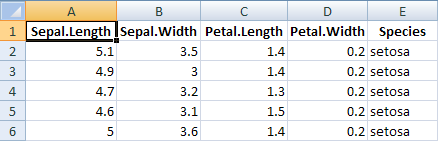
\includegraphics[height=1.7cm, keepaspectratio]{figures/iris_xlsx_3.png}
    \end{figure}
\end{center}
\end{frame}


\subsection{Le package xlsx: ajoût de tableaux}
\begin{frame}[containsverbatim]{Le package xlsx: création et ajoût de tableaux}
\par{Création d'un fichier Excel \Excel{} contenant deux tableaux dans la même feuille:}
\vspace{-2ex}
\begin{lstlisting}[language=R]
R> numericSummary <- data.frame(t(apply(iris[, 1:4], 2, quantile, seq(0, 1, 0.25))), check.names = FALSE)
R> wb <- createWorkbook(type = "xlsx")
R> sheet <- createSheet(wb, sheetName = "IRIS")
R> titleStyle <- CellStyle(wb,
       font = Font(wb, isBold = TRUE),
       alignment = Alignment(horizontal = "ALIGN_CENTER")
   )
\end{lstlisting}
\vspace{-2ex}
\begin{lstlisting}[language=R]
R> addDataFrame(iris, sheet, row.names = FALSE, colnamesStyle = titleStyle) # premier tableau
R> addDataFrame(numericSummary, sheet, startColumn = ncol(iris)+2, colnamesStyle = titleStyle, rownamesStyle = titleStyle) # second tableau
\end{lstlisting}
\vspace{-2ex}
\begin{lstlisting}[language=R]
R> autoSizeColumn(sheet, colIndex = seq(ncol(iris)+2+ncol(numericSummary)+1))
R> saveWorkbook(wb, file = "iris.xlsx")
\end{lstlisting}
\vspace{1ex}
\begin{center}
    \begin{figure}
        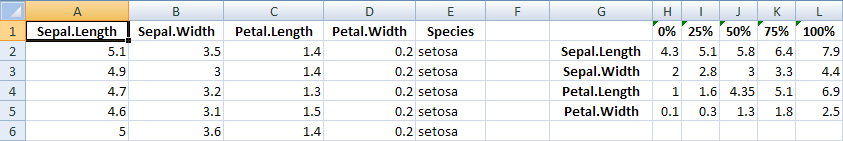
\includegraphics[height=1.7cm, keepaspectratio]{figures/iris_xlsx_4.png}
    \end{figure}
\end{center}
\end{frame}


\section{Générer un rapport}
\subsection{La syntaxe Markdown}
\begin{frame}[containsverbatim]{La syntaxe Markdown: écrire en Markdown I}
\par{La syntaxe Markdown utilise des combinaisons de symboles pour mettre en forme le texte: \cmdb{*}, \cmdb{-}, \cmdb{\#}, \cmdb{\_}, ...}
\vspace{-3ex}
\begin{multicols}{2}
\begin{lstlisting}[language=md, xleftmargin=9mm, xrightmargin=2mm, lineskip=5ex]
Texte normal
*italique* et _italique_
**gras** et __gras__
Exposant^2^
[un lien hypertexte](http://www-good.ibl.fr)
# Titre 1
## Titre 2
###### Titre 6
Equation: $A = \pi*r^{2}$
Image: ![](/path/logo_R.png)
\end{lstlisting}
\columnbreak
\vspace*{0.5ex}
\hspace{1cm}{\tiny Texte normal}\\
\hspace{1cm}{\tiny \textit{italique} et \textit{italique}}\\
\hspace{1cm}{\tiny \textbf{gras} et \textbf{gras}}\\
\hspace{1cm}{\tiny $Exposant^2$}\\
\hspace{1cm}{\tiny \href{http://www-good.ibl.fr}{un lien hypertexte}}\\
\hspace{1cm}{\large\textbf{Titre 1}}\\
\hspace{1cm}{\normalsize\textbf{Titre 2}}\\
\hspace{1cm}{\tiny\textbf{Titre 6}}\\
\hspace{1cm}{\tiny Equation: $A = \pi*r^{2}$}\\
\hspace{1cm}{\tiny Image: \R}\\
\end{multicols}
\end{frame}


\begin{frame}[containsverbatim]{La syntaxe Markdown: écrire en Markdown II}
\vspace{-3ex}
\begin{multicols}{2}
\begin{lstlisting}[language=md, xleftmargin=9mm, xrightmargin=2mm, lineskip=0ex]
* Liste à puces
    + item 1
    + item 2
\end{lstlisting}
\vfill
\columnbreak
\vspace*{\fill}
\begin{itemize}
\item \tiny Liste à puces
    \begin{itemize}
        \item \tiny sous item 1
        \item \tiny sous item 2
    \end{itemize}
\end{itemize}
\end{multicols}

\begin{multicols}{2}
\begin{lstlisting}[language=md, xleftmargin=9mm, xrightmargin=2mm, lineskip=0ex]
1. Liste à numéros
    + item 1
    + item 2
\end{lstlisting}
\vfill
\columnbreak
\vspace*{\fill}
\begin{enumerate}
    \item \tiny Liste à numéros
    \begin{itemize}
        \item \tiny sous item 1
        \item \tiny sous item 2
    \end{itemize}
\end{enumerate}
\end{multicols}

\begin{multicols}{2}
\begin{lstlisting}[language=md, xleftmargin=9mm, xrightmargin=2mm, lineskip=0ex]
Colonne 1 | Colonne 2
----------|----------
Cellule 1 | Cellule 2
Cellule 3 | Cellule 4
\end{lstlisting}
% \vfill
\columnbreak
\vspace*{2ex}
{\tiny
\begin{tabular}{l|l}
    Colonne 1 & Colonne 2 \\
    \hline
    Cellule 1 & Cellule 2\\
    Cellule 3 & Cellule 4\\
\end{tabular}
}
\end{multicols}
\end{frame}


\subsection{Le package rmarkdown: du R dans Markdown}
\begin{frame}[containsverbatim]{Le package rmarkdown: du \R{} dans Markdown}
\par{Le script au format Markdown s'écrit dans un fichier \cmdb{.rmd}. \\Le code \R{} s'écrit en ligne \cmdb{`r `} ou dans un block délimité par \cmdb{`}\cmdb{`}\cmdb{`\{\}} et \cmdb{`}\cmdb{`}\cmdb{`}.}
\vspace{-3ex}
\begin{multicols}{2}
\begin{lstlisting}[language=md, xleftmargin=9mm, xrightmargin=2mm, lineskip=0ex, aboveskip=0ex]
```{r}
a <- 1 + 1
a + 2
```
\end{lstlisting}
\columnbreak
\begin{lstlisting}[language=R, xleftmargin=2mm, xrightmargin=9mm, lineskip=0ex]
a <- 1 + 1
a + 2
\end{lstlisting}
\vspace{-3ex}
\begin{lstlisting}[language=Rconsole, xleftmargin=2mm, xrightmargin=9mm, lineskip=0ex]
[1] 4
\end{lstlisting}
\end{multicols}
\vspace{-6ex}
\begin{multicols}{2}
\begin{lstlisting}[language=md, xleftmargin=9mm, xrightmargin=2mm, lineskip=0ex, aboveskip=0ex]
```{r eval=TRUE, echo=FALSE}
a <- 1 + 1
a + 2
```
\end{lstlisting}
\columnbreak
\begin{lstlisting}[language=Rconsole, xleftmargin=2mm, xrightmargin=9mm, lineskip=0ex]
[1] 4
\end{lstlisting}
\end{multicols}
\par{Plusieurs options sont disponibles pour gérer les sorties graphiques et les résultats d'éxecution:\\
\quad \cmdb{dev}, \cmdb{dpi}, \cmdb{fig.cap}, \cmdb{fig.height}, \cmdb{fig.width}, \cmdb{fig.align}, \cmdb{cache}, \cmdb{results}, \cmdb{size}, ...\\}
% \par{{\footnotesize \href{http://rmarkdown.rstudio.com/RMarkdownReferenceGuide.pdf}{Petit guide pour R Markdown disponible ici!}}}
\end{frame}


\subsection{Le package rmarkdown: compiler un fichier .rmd}
\begin{frame}[containsverbatim]{Le package rmarkdown: compiler un fichier \cmdb{.rmd}}
\par{La compilation du code \R{} s'efectue avec le package \cmdb{knitr} (sans \cmdb{Pandoc}, le Markdown est convertis en html).}
\vspace{-2ex}
\begin{lstlisting}[language=R, lineskip=0ex]
R> library(rmarkdown)
R> knit2html("example.Rmd")
R> render("example.Rmd", output_format = "html_document")
R> render("example.Rmd", output_format = "all") # tout les formats definis dans le fichier
\end{lstlisting}
\vspace{-3ex}
\begin{multicols}{2}
\begin{lstlisting}[language=md, xleftmargin=9mm, xrightmargin=2mm, lineskip=0ex]
# Un titre en Markdown

## Un titre de sous niveau

Sinon on peut faire des calculs avec **R** comme 1 + 1 = `r 1 + 1`.
*Vous ne croyez tout de même pas que j'ai fait le calcul moi-même, si?*

```{r}
a <- 1 + 1
a + 2
```
\end{lstlisting}
\vfill
\columnbreak
\vspace*{\fill}
{\large\textbf{1 Un titre en Markdown}}\\\vspace{1ex}
{\normalsize\textbf{1.1 Un titre de sous niveau}}\\\vspace{1ex}
{\tiny Sinon on peut faire des calculs avec \textbf{R} comme 1 + 1 = 2.\\}\vspace{-1ex}
{\tiny \emph{Vous ne croyez tout de même pas que j'ai fait le calcul moi-même, si?}}
\vspace{-3ex}
\begin{lstlisting}[xleftmargin=2mm, xrightmargin=9mm, backgroundcolor=\color{white}, rulecolor=\color{white}, lineskip=0ex]
a <- 1 + 1
a + 2
[1] 4
\end{lstlisting}
\end{multicols}
\end{frame}


\subsection{Le package rmarkdown: ajouter un thème}
\begin{frame}[containsverbatim]{Le package rmarkdown: ajouter un thème (\cmdb{Pandoc})}
\par{Un thème peut également être appliqué:
\begin{itemize}
\item html : feuille de style css
\item \LaTeX{} (pdf / tex) : document format \LaTeX
\item Word \Word{} (docx) : document Word (provenant de pandoc)
\end{itemize}
}
\vspace{-2ex}
\begin{multicols}{2}
\begin{lstlisting}[language=md, xleftmargin=9mm, xrightmargin=2mm, lineskip=0ex]
# Un titre en Markdown

## Un titre de sous niveau

Sinon on peut faire des calculs avec **R** comme 1 + 1 = `r 1 + 1`.
*Vous ne croyez tout de même pas que j'ai fait le calcul moi-même, si?*

```{r}
a <- 1 + 1
a + 2
```
\end{lstlisting}
\vfill
\columnbreak
\vspace*{\fill}
{\large\textbf{{\color{dodgerblue}1 Un titre en Markdown}}}\\\vspace{1ex}
{\normalsize\textbf{{\color{dodgerblue}1.1 Un titre de sous niveau}}}\\\vspace{1ex}
{\tiny Sinon on peut faire des calculs avec \textbf{R} comme 1 + 1 = 2.\\}\vspace{-1ex}
{\tiny \emph{Vous ne croyez tout de même pas que j'ai fait le calcul moi-même, si?}}
\vspace{-3ex}
\begin{lstlisting}[language=R, xleftmargin=2mm, xrightmargin=9mm, lineskip=0ex]
a <- 1 + 1
a + 2
\end{lstlisting}
\vspace{-3ex}
\begin{lstlisting}[language=Rconsole, xleftmargin=2mm, xrightmargin=9mm, lineskip=0ex]
[1] 4
\end{lstlisting}
\end{multicols}
\end{frame}


\begin{frame}[containsverbatim]{Le package rmarkdown: ajouter un thème (\cmdb{YAML})}
\par{Les thèmes sont définis au préalable dans des fichiers séparés qu'il faut importer dans le format \href{http://fr.wikipedia.org/wiki/YAML}{YAML} au début du fichier \cmdb{.rmd}}
\vspace{-2ex}
\begin{lstlisting}[language=yaml, lineskip=0ex]
---
output:
    word_document:
        pandoc_args: [
            "--reference-docx=votreTheme.docx"
        ]
    html_document:
        theme: cerulean <!-- plusieurs theme de couleurs sont disponibles-->
        css: votreTheme.css
    pdf_document:
        template: votreTheme.tex
    beamer_presentation:
        template: votreTheme.tex
---
\end{lstlisting}
\par{
\begin{itemize}
    \item \href{http://bootswatch.com/}{bootswatch.com}: gallerie de thèmes css.
    \item \href{https://github.com/jgm/pandoc-templates}{github.com/jgm/pandoc-templates}: thème pandoc par défaut.
\end{itemize}
}
\end{frame}


\subsection{Le package rmarkdown: les options Pandoc}
\begin{frame}[containsverbatim]{Le package rmarkdown: les options \cmdb{Pandoc}}
\par{Plusieurs paramètres peuvent être définis via l'entête \href{http://fr.wikipedia.org/wiki/YAML}{YAML} pour générer des documents \LaTeX:
\vspace{-2ex}
\begin{multicols}{2}
\begin{itemize}
    \item \cmdb{lang}
    \item \cmdb{fontsize}
    \item \cmdb{documentclass}
    \item \cmdb{geometry}
    \columnbreak
    \item \cmdb{number\_sections}
    \item \cmdb{toc}
    \item \cmdb{keep\_tex}
    \item \cmdb{pandoc\_args}
\end{itemize}
\end{multicols}
}
\vspace{-4ex}
\begin{lstlisting}[language=yaml, lineskip=0ex]
---
output:
    pdf_document:
        number_sections: true
        toc: true
        keep_tex: true
        template: votreTheme.tex
        pandoc_args: [
            "--listings" <!-- Utilise l'environnement listings pour le code -->
        ]
---
\end{lstlisting}
\end{frame}


\subsection{Le package rmarkdown: ça donne ça!}
\begin{frame}{Le package rmarkdown: \LaTeX{} article (\cmdb{pdf})}
\begin{center}
    \begin{figure}
        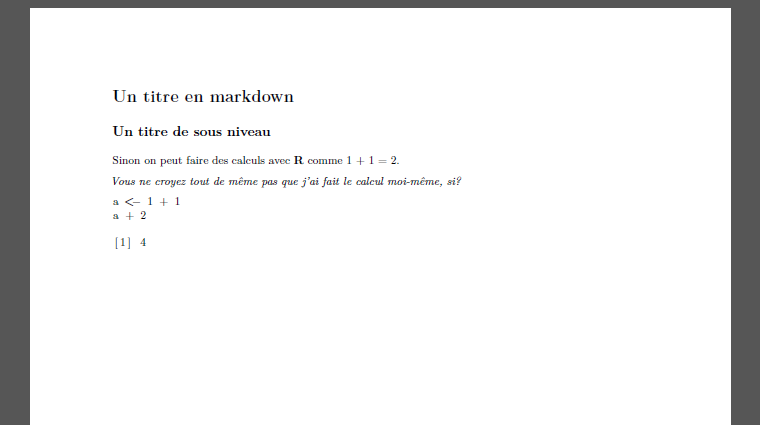
\includegraphics[width=0.75\paperwidth, keepaspectratio]{figures/article.png}
    \end{figure}
\end{center}
\end{frame}

\begin{frame}{Le package rmarkdown: word (\cmdb{docx})}
\begin{center}
    \begin{figure}
        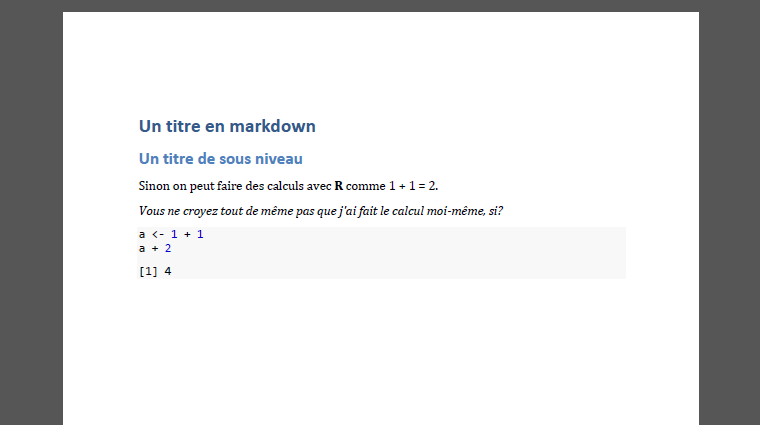
\includegraphics[width=0.75\paperwidth, keepaspectratio]{figures/word.png}
    \end{figure}
\end{center}
\end{frame}

\begin{frame}{Le package rmarkdown: \cmdb{html}}
\begin{center}
    \begin{figure}
        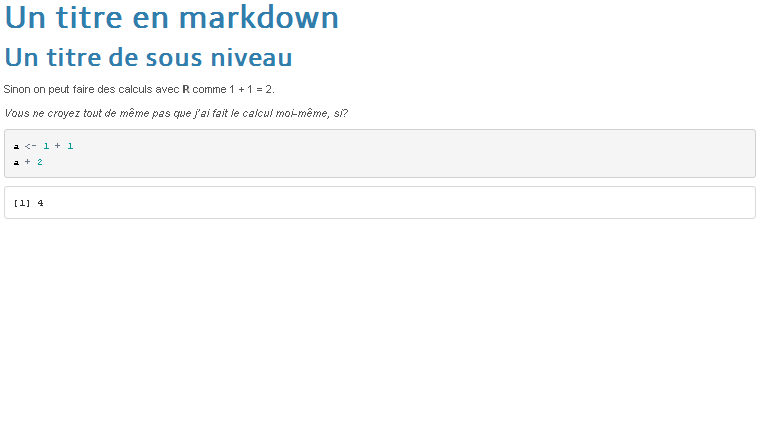
\includegraphics[width=0.75\paperwidth, keepaspectratio]{figures/html.png}
    \end{figure}
\end{center}
\end{frame}

\begin{frame}{Le package rmarkdown: \LaTeX{} beamer (\cmdb{pdf})}
\begin{center}
    \begin{table}
        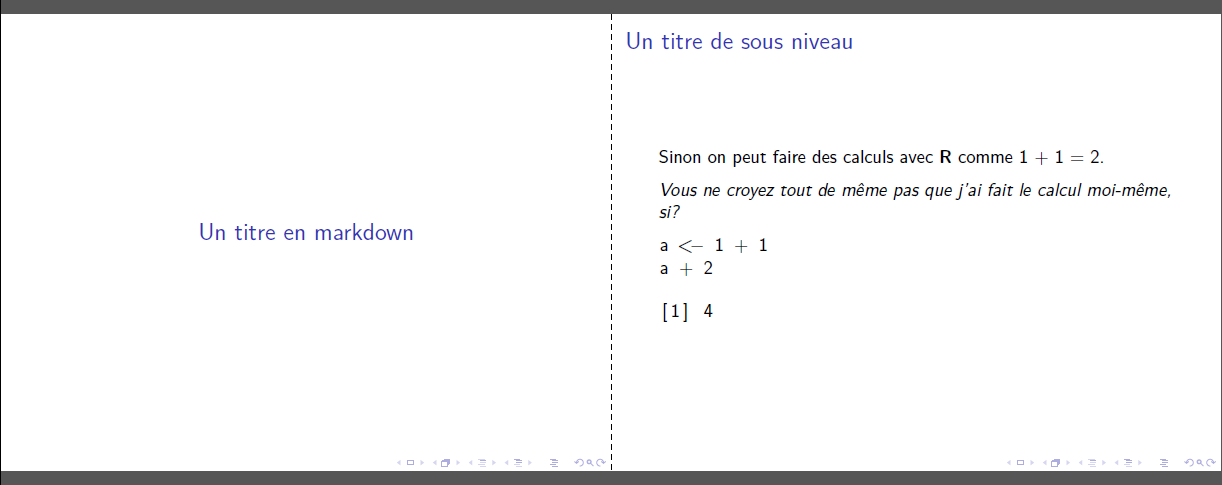
\includegraphics[width=0.75\paperwidth, keepaspectratio]{figures/beamer.png}
    \end{table}
\end{center}
\end{frame}


\section{References}
\begin{frame}{References}%[allowframebreaks]
    \bibliographystyle{apalike}
    \bibliography{MARKDOWN_biblio.bib}
    \nocite{*}
\end{frame}

\end{document}